\subsection{Boxplots}
In the following section we will discuss what the boxplots of the attributes tell us about the data.
Below is a figure representing the boxplot for the referenced attribute.
\begin{figure}[H]
\centering
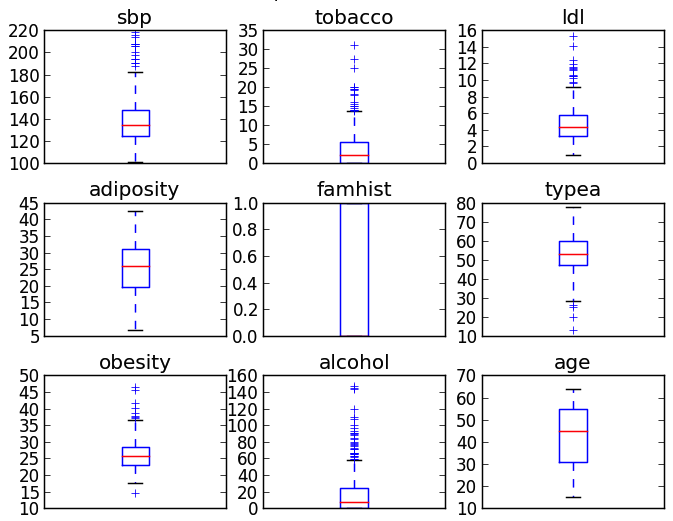
\includegraphics[width=12cm, keepaspectratio=true]{pictures/boxplot.png}
\caption{\footnotesize Boxplots}
\label{boxplot}
\end{figure}
\paragraph{SBP - Systolic Blood Pressure} shows us that most of the measured blood pressure is close to 130 mmHg. However, we see that there is a lot of outliers in the dataset. This raises a bit of suspicion, since the amount of outliers is quite high. According to other sources \footnote{http://en.wikipedia.org/wiki/Blood\_pressure}, when the blood pressure rises above 180 mmHg for a longer period of time, organs will start to fail. This could indicate that some of the data are incorrect.

SKRIV HER HVOR MANGE DER LIGGER OVER 180!!!

\paragraph{Tobacco consumption} is another boxplot which is showing a large amount of outliers in the data. This time however, it is not necessarily bad data, but just a higher level of use. Since it is based on the total amount of tobacco in kilos, used over the persons life time, it is expected to see some very high values at people who started smoking early, and is older than the average.

\paragraph{ldl - low density lipoprotein cholesterol} is measured in mmol/L. Anything above 4.9 is considered a high cholesterol \footnote{http://www.mayoclinic.com/health/cholesterol-levels/CL00001}. This seems to be consistent with the data from the boxplot. But again there is a large amount of outliers, and it does seem odd to have an ldl value more than tripple what is considered to be high.

IGEN SKRIV HVOR MANGE DET DREJER SIG OM!!

\paragraph{Adiposity} is an index number to group people by their size, much like BMI. The boxplot shows no outliers, and the average is consistent with what is considered to be normal. \footnote{http://easycalculation.com/health/body-adiposity-index.php}

\paragraph{Famhist} is a binary value, and does not tell us anything useful in a boxplot. Off to the next attribute.

\paragraph{TypeA} is an indicator to show aggresiveness of a person, based on an evaluation. Even though there are outliers in the boxplot, we do not consider those as suspicious, as the index ranges from 0 to 100.

\paragraph{Obesity - BMI} is another indicator of the persons size, much like the adiposity index, just calculated a bit different. Since the adiposity and BMI index is closely correlated (as shown later) we do not consider the outliers to be a concern. The outliers do still lie within a plausible BMI value.

\paragraph{Alcohol} contains a lot of outliers. Most of the readings from the dataset shows an alcohol consumption of 0, or nearly 0, which makes the average consumption almost 0. This causes the overall maximum to be low, and by then creating a lot of outliers. We do not consider these outliers a concern, since it is well known, that some have a considerably higher alcohol consumption level than average.

\paragraph{Age} does not show us any really useful in a boxplot, except for the fact that the age range goes from around 15 to 65.

